\documentclass[11pt]{beamer}
\usetheme{Warsaw}
\usepackage[utf8]{inputenc}
\usepackage[spanish]{babel}
\usepackage{amsmath,amsthm,amssymb} %modos matemáticos y  simbolos
\usepackage{latexsym,amsfonts} %simbolos matematicos
\usepackage{graphicx}
\usepackage{physics} %Simbolos fisicos
\usepackage{array} %mejores formatos de tabla
\usepackage{tabulary}
\usepackage{multirow} %ocupar varias filas en una tabla
\usepackage{fancybox} %recuadros talegas
\usepackage{float} %ubicar graficas
\usepackage{color}
\usepackage{comment}
\usepackage{stackrel}
\usepackage{calligra}
\usepackage{lipsum} % texto de relleno
\usepackage{cite}
\author{Diego Sarceño}
\title{Tiro Parabólico}
%\setbeamercovered{transparent} 
%\setbeamertemplate{navigation symbols}{} 
%\logo{} 
\institute{\footnotesize{201900109} \\ Escuela de Ciencias Físicas y Matemáticas} 
\date{\today} 
%\subject{Capítulo $3.1.1.$} 
\begin{document}

\begin{frame}
\titlepage
\end{frame}

%\begin{frame}
%\tableofcontents
%\end{frame}

%\AtBeginSection[]
%{
%    \begin{frame}<beamer>{Contenido}
%        \tableofcontents[currentsection]
%    \end{frame}
%}

\frame{
    \frametitle{Contenido}
    \tableofcontents
}
%%%%%%%%%%%%%%%%%%%%%%%%%%%%%%%%%%%%%%%%%%%%%%%%%%%%%%%%%
%---------------Movimiento parabolico--------------------
\section{Movimiento Parabólico}
\frame{
	\frametitle{Recordatorio}
    Anteriormente se estudio a una particula moviendose a velocidad constante (MRU) y a aceleración constante (MRUV); en concreto, nos intereso el movimiento de caída libre.
    
}

\frame{
    \frametitle{Recordatorio}
    Las ecuaciones que modelan dichos dos movimientos son:
    \begin{enumerate}
        \item MRU 
        \begin{align*}
            \vec{v} &=\frac{\Delta \vec{x}}{\Delta t} \\
            x_f &=x_o +vt
        \end{align*}
        \item MRUV
        \begin{align*}
            \vec{a} &=\frac{\Delta \vec{v}}{\Delta t} \\
            v_f &=v_o +at \\
            v_f ^2 &=v_o ^2 +2a\Delta x \\
            \Delta x &=\qty(\frac{v_f +v_o }{2})t \\
            x_f &=x_o +v_o t +\frac{1}{2} at^2
        \end{align*}
    \end{enumerate}
}

\frame{
    \frametitle{Movivmiento Parabólico}
    Este tipo específico de movimiento se da si la resistencia del aire es despreciable. Comúnmente se le denomina movimiento de proyectiles.
}

\frame{
    \frametitle{Características}
    \begin{block}{Definición}
        El movimiento parabólico es una combinación de dos tipos de movimientos ya conocidos.
        \begin{itemize}
            \item Movimiento con velocidad constante. El cual es el movimiento que presenta la particula en el eje horizontal.
            \item Movimiento con aceleración constante ($g$). El cual es el que presenta la particula en el eje vertical.
        \end{itemize}
        Ambos movimientos combinados generan el movimiento de proyectiles (parabólico).
    \end{block}
}
\frame{
    \frametitle{Modelo del Movimiento}
    \begin{figure}[H]
        \centering
        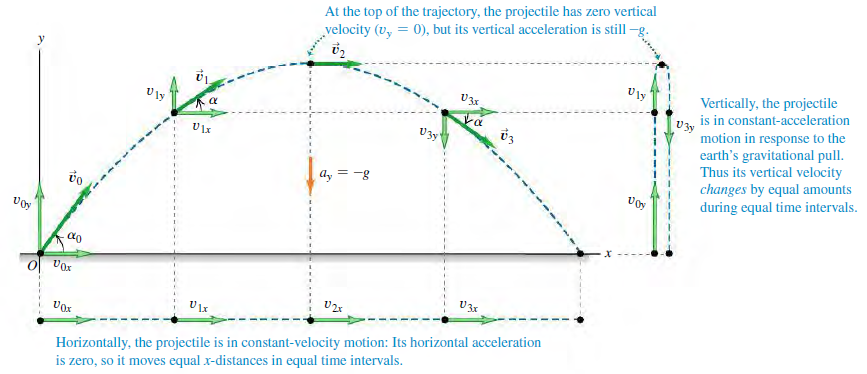
\includegraphics[scale=0.5]{img/PROY.PNG}
        \caption{Figura $3.17$, Zemansky 14$-$Ed}
        \label{PROYECTILES}
    \end{figure}
}

\frame{
    \frametitle{Modelo del Movimiento}
    Notese que en este caso no tenemos la velocidad inicial en ninguno de los dos ejes, sino, para que el movimiento exista, debe de ser una velocidad a cierto ángulo respecto la horizontal (o vertical). En la figura \ref{PROYECTILES} vemos que para poder modelar el movimiento vertical y horizontal requerimos descomponer la velocidad en ambas componentes, es claro ver que dichas componentes son:
    \begin{align*}
        v_x &=v_o \cos{\alpha _o} \\
        v_y &=v_o \sin{\alpha _o}
    \end{align*}
    Esto es cierto si y solo si el ángulo es medido respecto de la horizontal.
}

\frame{
	\frametitle{Ejemplo 1: } 
	Encontraremos la ecuación que genere la parábola característica de dicho movimiento: 
}

\frame{
    \frametitle{Alcance Horizontal y Altura Máxima}
    Esto es una carcterística especifica del movimiento parabólico (cuando el proyectil llega al nivel del suelo).
    El alcance horizontal es la distancia que le proyectil alcanza horizontalmente:
    \begin{align*}
        \chi &=\frac{v_o ^2 \sin{2\alpha}}{g}
    \end{align*}
    Y la altura máxima es alcanzada cuando la velocidad en $y$ es cero:
    \begin{align*}
        H_{max} &=\frac{v_o ^2 \sin ^2 {\alpha _o}}{2g}
    \end{align*}
    
}

\frame{
    \frametitle{Alcance Horizontal}
    En superficies planas, si tenemos la misma velocidad inicial, existen ángulos a los cuales los proyectiles tienen el mismo alcance horizontal. Los ángulos complementarios, bajo la misma velocidad inicial, tienen el mismo alcance horizontal. (La demostración es un ejercicio de la hoja de trabajo)
    
}

\frame{
	\frametitle{Ejemplo 2: }
	Un libro de física que se desliza sobre una mesa horizontal a $1.10 \flatfrac{m}{s}$ cae y llega al piso en $0.350 s$. Ignore la resistencia del aire.
        Calcule $a)$ la altura de la mesa con respecto al piso; $b)$ la distancia horizontal del borde de la mesa al punto donde cae el libro.
}

%%%%%%%%%%%%%%%%%%%%%%%%%%%%%%%%%%%%%%%%%%%%%%%%%%%%%%%%%
%--------------Movimiento Circular Uniforme--------------



\frame{
	\centering
	\vspace{1cm}
	GRACIAS POR SU ATENCIÓN
}














\end{document}